\section{Rubin Observatory Commissioning}
\label{sec:commissioning}

\subsection{Commissioning Plan and Schedule}
\label{ssec:commissioning-schedule}

Figure~\ref{fig:commissioning-es-schedule} shows the detailed schedule of commissioning and early science activities relative to System First Light, as of \currentdate.
\begin{figure}[htb]
\centering
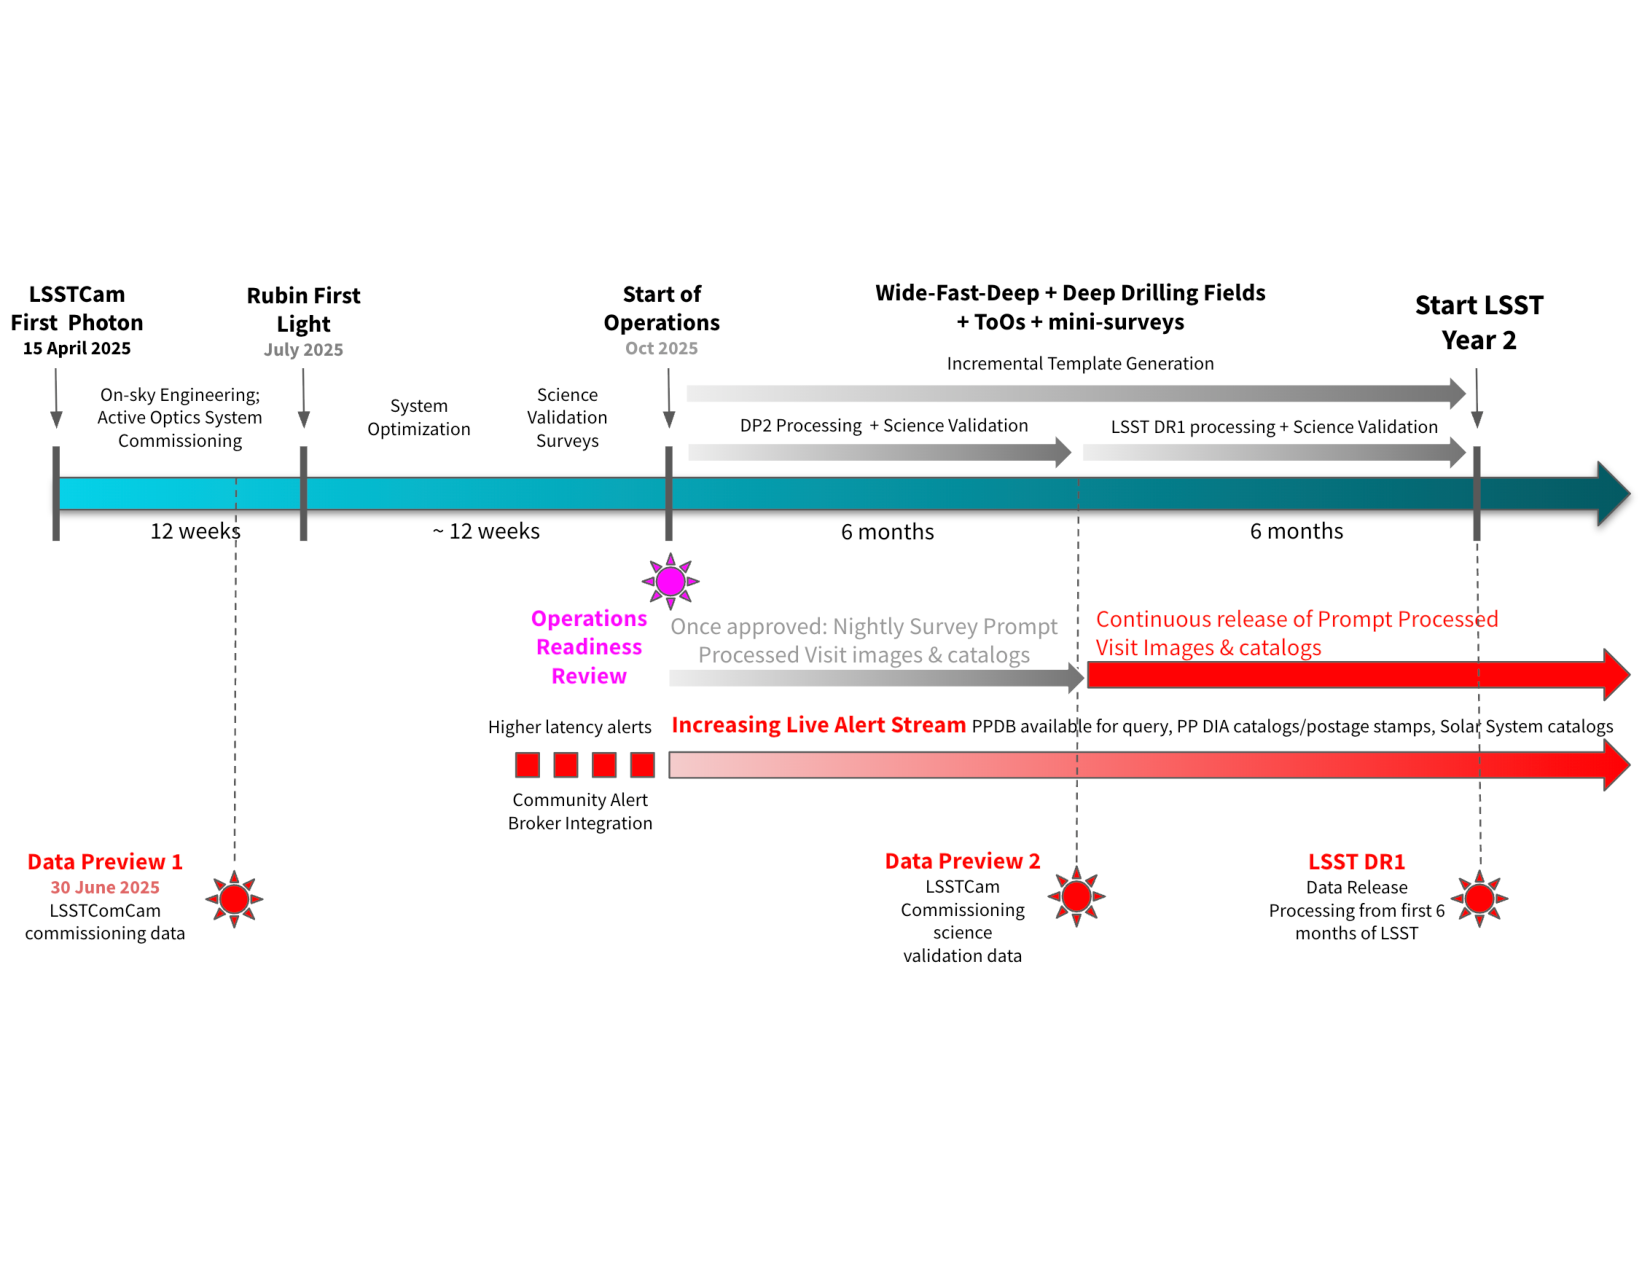
\includegraphics[width=0.98\linewidth]{figures/rubinobs_on-sky_commissioning_and_early_science.pdf}
\caption{Detailed schedule of commissioning  and early science activities relative to System First Light, as of \currentdate.}
\label{fig:commissioning-es-schedule}
\vspace{0.1cm}
\end{figure}
ComCam First Photon was successfully achieved on 24 October 2024.
Rubin (LSSTCam) First Photon, is currently expected on 15 April 2025 and System First Light in  July 2025 (\S~\ref{sec:timeline}). 

Figure~\ref{fig:commissioning} shows the high level plan for the Rubin commissioning observations. 
\begin{figure}[htb]
\centering
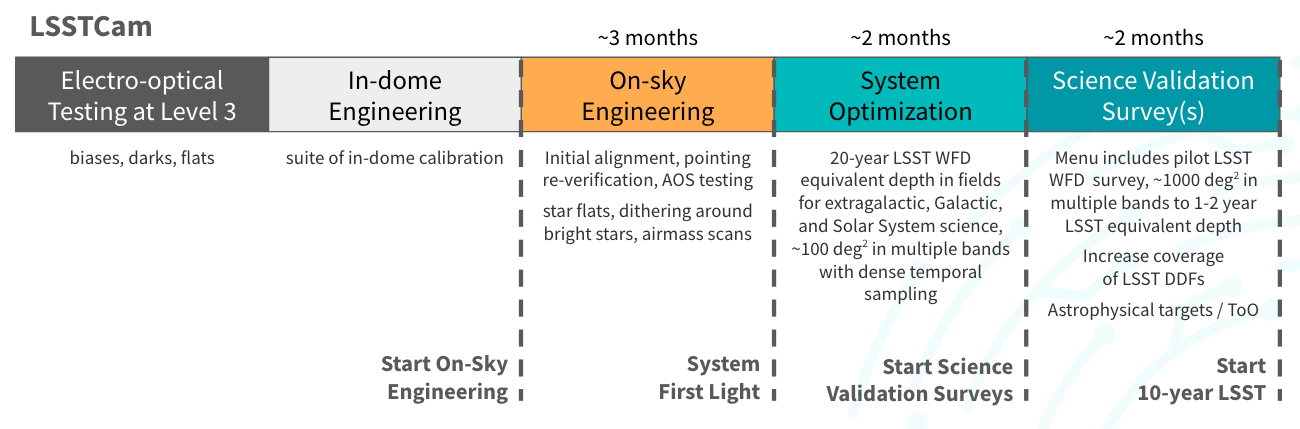
\includegraphics[width=0.95\linewidth]{figures/commissioning-plan}
\caption{Outline plan for the collection of commissioning data, as of \currentdate.}
\label{fig:commissioning}
\end{figure}
Commissioning data collection is planned to take place in phases.
The On-Sky Engineering phase may be carried out with either ComCam and/or LSSTCam, depending on the optimal sequence of integration activities.
Both the System Optimization and Science Validation (SV) phases are carried out with LSSTCam. 
The System Optimization phase will collect a set of observations designed to help optimize the system prior to starting the Science Validation phase.
During the Science Validation phase, a series of SV Surveys designed to support scientific analyses that validate the system's performance and allow Rubin to demonstrate operations readiness are carried out, see \citeds{SITCOMTN-005}.
The System Optimization and SV phases contain a number of planned key components, including an LSST wide-fast-deep (WFD) 1-2 year equivalent depth ``pilot'' survey.
In all phases, field selection will be carried out by the commissioning team, taking into account a wide variety of constraints as well as a ``menu'' of science opportunities to which the LSST Science Community has contributed.

The System Optimization and SV survey phases are expected to last about 8 weeks each.
The project schedule will continue to evolve as the remaining subcomponents are delivered. 
Construction is expected to complete and LSST data taking start before the end of 2026.

\subsection{Commissioning Milestones}
\label{ssec:commissioning-milestones}

Commissioning work is being planned around three major milestones, \textit{ComCam First Photon}, \textit{LSSTCam First Photon} and \textit{System First Light}. 

\textbf{ComCam First Photon}: The first image of the night sky produced by photons passing through the Rubin optical system and detected by the Commissioning Camera (ComCam). 
This milestone was achieved on 24 October 2024. 

\textbf {LSSTCam First Photon}: The first image of the night sky produced by photons passing through the Rubin optical system and detected by the LSST Science Camera (LSSTCam).
Currently expected  for 15 April 2025.

\textbf {System First Light}: Defined as the point at which we can routinely acquire science-grade imaging across the LSSTCam full focal plane and have a well understood technical path towards meeting the Construction Completeness criteria   \citeds{sitcomtn-061}.
Currently expected for 4 July 2025. 

LSSTCam First Photon occurs following the successful completion of system integration. 
There are no quality criteria applied to achieving  neither the ComCam nor LSSTCam First Photon milestones. 
System First Light  marks the end of the  on-sky engineering phase and the start of the System Optimization and Science Validation phases of commissioning.
The period between ComCam First Photon and System First Light will focus on fine tuning the system including optical alignment and improving the image quality and collecting calibration data.
For a detailed description of all the commissioning milestones and the most current dates, see \citeds{dmtn-232}.

\subsection{ComCam Commissioning }
\label{ssec:commissioning-comcam}

ComCam is Rubin's engineering camera that is used for testing and validating the observatory's systems and processes prior to installation of the LSST Camera.
The ComCam focal plane has single raft with a 3×3 mosaic of 4K×4K ITL science sensors, giving a total of 144Mpix. 
ComCam has the same plate scale as LSSTCam (0.2 arcsec / pixel), with a field of view of 40  × 40 arcmin. 
The ComCam filter exchanger holds only three physical filters at a time.

The Rubin on-sky commissioning campaign using ComCam began on 24 October 2024 and ended on 11 December 2024, lasting a total of 7 weeks, and included observations to support both engineering and science pipelines commissioning.
This highly successful campaign included a first series of on-sky engineering tests demonstrating the end-to-end functionality of the Simonyi Survey Telescope’s hardware and software systems ComCam.
The median delivered image quality  for commanded in-focus images collected during the campaign, quantified in terms of the PSF FWHM, was $\approx$1.1 arcseconds. 
The best images have delivered PSF FWHM of $\approx$0.7 arcseconds.
A full report on the ComCam on-sky commissioning campaign is available at \citeds{sitcomtn-149}.


\subsection{LSSTCam Commissioning }
\label{ssec:commissioning-lsstcam}

As of \currentdate, LSSTCam is being installed on the Simonyi Survey Telescope and on-sky observing is expected to begin in April 2025.

